\documentclass[fleqn,10pt]{project}


\definecolor{color1}{RGB}{0,0,90}
\definecolor{color2}{RGB}{0,20,20}

\usepackage{tcolorbox,listings,multirow,placeins,tikz,pgf,pdfpages, lipsum, pdflscape, pgfgantt}
\usepackage[normalem]{ulem}
\usetikzlibrary{shapes.geometric, arrows,shapes,positioning,shadows,trees}

\useunder{\uline}{\ul}{}

\tikzstyle{process} = [rectangle, minimum width=3cm, minimum height=1cm, text centered, draw=black, fill=blue!30]
\tikzstyle{arrow} = [thick,->,>=stealth]

\tikzset{
every node/.style={draw,text width=2cm,drop shadow},
style1/.style= {rectangle, rounded corners=2pt, thin,align=center,fill=green!30},
style2/.style= {rectangle, rounded corners=6pt, thin,align=center,fill=green!60},
style3/.style= {rectangle,thin,align=left,fill=pink!60}
}

\lstset{
	showstringspaces=false,
  tabsize=2,
  breaklines=true,
  columns=fullflexible
}
\tcbuselibrary{breakable}

\usepackage{hyperref}
\hypersetup{hidelinks,colorlinks,breaklinks=true,urlcolor=color2,citecolor=color1,linkcolor=color1,bookmarksopen=false,pdftitle={Title},pdfauthor={Author}}

\JournalInfo{

\includegraphics[width=2.5cm]{Figures/engineering-logo}
\Archive{}
}

\PaperTitle{Senior Design Project Report Template}

\Authors{First name Last Name\textsuperscript{1}*,
First Name Last Name\textsuperscript{1}**,
First Name Last Name\textsuperscript{1}***.}
\affiliation{\textsuperscript{1}\textit{Engineering, 
  University of Mary, Bismarck, North Dakota}}
\affiliation{*email@umary.edu}
\affiliation{**email@umary.edu}
\affiliation{***email@umary.edu}

\Keywords{}
\newcommand{\keywordname}{Keywords}
\Abstract{Give a one paragraph summary of the whole document.}
\begin{document}

\flushbottom
\maketitle
\tableofcontents
\thispagestyle{empty}

\section{Introduction}

Describes the problem domain and the specific problem to be resolved, 
reviews existing solutions and their inadequacies, and how the design project, 
adequately resolves the specific problem. 

\subsection{Statement of Project Qualifications}

The statement of qualifications shall be of the following format. This document should be accurate as possible at
the beginning of the project but it may require changes. All subsequent research, reports and status reports
should have a direct reference to this document.

% Please add the following required packages to your document preamble:
% \usepackage[table,xcdraw]{xcolor}
% Beamer presentation requires \usepackage{colortbl} instead of \usepackage[table,xcdraw]{xcolor}
\begin{table}[!h]
\begin{centering}
\begin{tabular}{|ll|}
\hline
\multicolumn{1}{|l|}{{\color[HTML]{FF0000} Project Name}}                     &                                                                                                                                                                                                                                                                                                                                                                                                                                                                                                            \\ \hline
\multicolumn{1}{|l|}{{\color[HTML]{FF0000} Project Members}}                  &                                                                                                                                                                                                                                                                                                                                                                                                                                                                                                            \\ \hline
\multicolumn{1}{|l|}{{\color[HTML]{FF0000} Stakeholders}}                     & \begin{tabular}[c]{@{}l@{}}A project stakeholders is a person or an organization that is actively involved in the project \\ or that is positively or negatively impacted by it. e.g. they control or influence the project \\ budget,they provide permission to proceed, they directly benefit from or are impacted by \\ the project,they remove roadblocks or exert influence when needed to ensure project \\ success, or their positive or negative energy could affect project success.\end{tabular} \\ \hline
\multicolumn{1}{|l|}{{\color[HTML]{FF0000} Project Purpose}}                  & \begin{tabular}[c]{@{}l@{}}The purpose of the project is its motivations (there may be several).  For instance a company \\ might design a product to increase market share.   A project might be undertaken to help \\ the disabled.  As students, part of your motivation is educational.  You learn more about \\ product design through a simulated design experience in class and also learn more about a \\ technical area of interest.\end{tabular}                                                   \\ \hline
\multicolumn{1}{|l|}{{\color[HTML]{FF0000} Description}}                      & \begin{tabular}[c]{@{}l@{}}Give an explanation broadly of what your project is and then the work that the project will \\ involve.\end{tabular}                                                                                                                                                                                                                                                                                                                                                            \\ \hline
\multicolumn{1}{|l|}{{\color[HTML]{FF0000} Desired Results}}                  & \begin{tabular}[c]{@{}l@{}}Give your goals for the project.  These goals should be specific, measurable, relevant to the \\ project, and achievable with-in the semester.\end{tabular}                                                                                                                                                                                                                                                                                                                     \\ \hline
\multicolumn{1}{|l|}{{\color[HTML]{FF0000} Exclusions}}                       & \begin{tabular}[c]{@{}l@{}}Here specifically state things that are beyond the scope of the project and types of work\\  that you will not engage in, in this project but which are conceivably relevant to it.\end{tabular}                                                                                                                                                                                                                                                                                \\ \hline
\multicolumn{1}{|l|}{{\color[HTML]{FF0000} Communication Needs}}              & \begin{tabular}[c]{@{}l@{}}Explain what information needs to be communicated between project members and project \\ members and instructors for the success of the project.\end{tabular}                                                                                                                                                                                                                                                                                                                    \\ \hline
\multicolumn{1}{|l|}{{\color[HTML]{FF0000} Acceptance Criteria}}              & \begin{tabular}[c]{@{}l@{}}One acceptance criteria for the project is approval of the course instructors.  You may have\\ more acceptance criteria if you have multiple stakeholders.\end{tabular}                                                                                                                                                                                                                                                                                                         \\ \hline
\multicolumn{1}{|l|}{{\color[HTML]{FF0000} Constraints}}                      & \begin{tabular}[c]{@{}l@{}}Here describe the types of constrains that are most relevant to your project. For instance, \\ manufacturability/constructability, maintainability, safety, environmental impact, \\ and cost are important considerations for all engineering projects but will vary in relative \\ level of priority depending on the nature of the project.\end{tabular}                                                                                                                    \\ \hline
\multicolumn{2}{|c|}{{\color[HTML]{FF0000} High Level Assignments}}                                                                                                                                                                                                                                                                                                                                                                                                                                                                                                                        \\ \hline
\multicolumn{1}{|l|}{{\color[HTML]{FF0000} \textless{}Student\textgreater{}}} & Here describe the work that every member of your group will be engaged in.                                                                                                                                                                                                                                                                                                                                                                                                                                 \\ \hline
\multicolumn{1}{|l|}{{\color[HTML]{FF0000} \textless{}Student\textgreater{}}} &                                                                                                                                                                                                                                                                                                                                                                                                                                                                                                            \\ \hline
\multicolumn{1}{|l|}{{\color[HTML]{FF0000} \textless{}Student\textgreater{}}} &                                                                                                                                                                                                                                                                                                                                                                                                                                                                                                            \\ \hline
\multicolumn{1}{|l|}{{\color[HTML]{FF0000} \textless{}Student\textgreater{}}} &                                                                                                                                                                                                                                                                                                                                                                                                                                                                                                            \\ \hline
\end{tabular}
\end{centering}
\end{table}

\subsection{Background and motivation}

This section must always include a literature review.  The background section gives a narrative giving an extensive description of what the need is
that motivates the project, what some potential solutions are, and any other important information. 
The background section is the fruit of your research. It should show that you understand the 
problem very very well and give the reader a robust qualitative explanation of it. For instance, 
the motivation for developing a quadcopter that can string power lines could go into the risks 
to manned crews and why a safer method is needed. It would go into alternative solutions to a 
quadcopter and why you think those can be dispensed with from the start in preference for a quadcopter based solution.

\subsection{Design Requirements}

\subsubsection{Functional Requirements / Product Specifications}

Describes the needs of the end user and translates those needs into technical 
requirements for the solution to the engineering problem adequate for the solution’s 
realization. These requirements are expressed as measurable specifications using 
explicit metrics and values adequate for testing. The specification discussion must 
address the standards and applied constraints applicable to the problem domain and 
proposed solution. The section shall also explain how each specification and its value 
was determined. 

\subsubsection{Additional Considerations}

Discusses the applied constraints, such as economic factors, safety, reliability, aesthetics, 
manufacturability/constructability, maintainability, environmental impact and sustainability,
ethics, and social impact, related to the completed product. Comparison of the understanding 
of applied constraints at the conclusion of the project to those that were considered during 
the design aspects of the project shall be included. 

\begin{landscape}
\subsection{Requirements Traceability Matrix}
The requirements traceability matrix does two things. The traceability matrix relates more 
specific, quantifiable technical requirements, to broader more qualitative requirements
that they are derived from.  For instance, if the broader requirement for a bridge is
that it must not fall down, a more specific requirement derived from this could be 
that the bridge must hold a live load of 10,000 lbs.  In turn, derived from that might be a
requirement for the tensile strength of the members of the truss and so on.  Additionally, 
the requirement traceability matrix specifies the method of requirement verification
as well as the specific deliverable that provides the verification. 

An example traceability matrix is provided below.  In the table below the ID is the 
designation you will use to refer to a requirement.  The category is the type of 
requirement it is. That is does it pertain to safety, functionality, manufacturability/constructability
cost, etc.. Requirement description is where you explain the requirement.  Priority is 
the level of importance of the requirement to the project.  Objective is what outcome / goal of 
the project the requirement pertains to.  Source specifies where the requirement comes from. Top
level requirements derive from the project qualification statement, what you agreed to do
at the start of the semester.  This is what your stakeholders are asking for.
Lower level requirements derive from higher level requirements. So the specific higher level requirement
is the  lower level requirements source.  The verification method is how you will verify that the 
requirement has been met.  Broadly speaking these methods are inspection, demonstration, testing, analysis,
and/or simulation.  For instance, you can inspect a part to make sure it doesn't have sharp edges.  You
can demonstrate that a vehicle can operate on certain terrain by building a prototype and operating it on
that terrain. You can test a welded rod in a UTM to verify its maximum load.  You can mathematically analyze
a truss to determine what the load in each member will be.  You could use FEA to simulate the loading of 
the frame of a bicycle to determine what the stress in the members will be.  Demonstrations and some
testing requires prototypes.  Analysis is done mathematically.  Simulations are also inherently
mathematical and therefore require that the user has some familiarity with the principles and assumptions
inherent in the simulation to be reliable. 

% Please add the following required packages to your document preamble:
% \usepackage{multirow}
\begin{table}[!h]
\centering
\begin{tabular}{|cccccccc|}
\hline
\multicolumn{8}{|c|}{REQUIREMENTS TRACEABILITY MATRIX}                                                                                                                                                                                                                                                                                                                                      \\ \hline
\multicolumn{1}{|c|}{\multirow{3}{*}{\begin{tabular}[c]{@{}c@{}}Project \\ Description\end{tabular}}} & \multicolumn{3}{c|}{\multirow{3}{*}{}}                                                                       & \multicolumn{2}{c|}{\multirow{3}{*}{\begin{tabular}[c]{@{}c@{}}Team  \\ Members\end{tabular}}} & \multicolumn{1}{c|}{}                    &                          \\ \cline{7-8} 
\multicolumn{1}{|c|}{}                                                                                & \multicolumn{3}{c|}{}                                                                                        & \multicolumn{2}{c|}{}                                                                          & \multicolumn{1}{c|}{}                    &                          \\ \cline{7-8} 
\multicolumn{1}{|c|}{}                                                                                & \multicolumn{3}{c|}{}                                                                                        & \multicolumn{2}{c|}{}                                                                          & \multicolumn{1}{c|}{}                    &                          \\ \hline
\multicolumn{1}{|c|}{}                                                                                & \multicolumn{1}{c|}{}         & \multicolumn{1}{c|}{}                        & \multicolumn{1}{c|}{}         & \multicolumn{1}{c|}{}                           & \multicolumn{1}{c|}{}                        & \multicolumn{1}{c|}{}                    &                          \\ \hline
\multicolumn{5}{|c|}{REQUIREMENT INFORMATION}                                                                                                                                                                                                                          & \multicolumn{3}{c|}{RELATIONSHIP TRACEABILITY}                                                                     \\ \hline
\multicolumn{1}{|c|}{ID}                                                                              & \multicolumn{1}{c|}{Category} & \multicolumn{1}{c|}{Requirement Description} & \multicolumn{1}{c|}{Priority} & \multicolumn{1}{c|}{Objective}                  & \multicolumn{1}{c|}{Source}                  & \multicolumn{1}{c|}{Verification Method} & Verification Deliverable \\ \hline
\multicolumn{1}{|c|}{}                                                                                & \multicolumn{1}{c|}{}         & \multicolumn{1}{c|}{}                        & \multicolumn{1}{c|}{}         & \multicolumn{1}{c|}{}                           & \multicolumn{1}{c|}{}                        & \multicolumn{1}{c|}{}                    &                          \\ \hline
\multicolumn{1}{|c|}{}                                                                                & \multicolumn{1}{c|}{}         & \multicolumn{1}{c|}{}                        & \multicolumn{1}{c|}{}         & \multicolumn{1}{c|}{}                           & \multicolumn{1}{c|}{}                        & \multicolumn{1}{c|}{}                    &                          \\ \hline
\multicolumn{1}{|c|}{}                                                                                & \multicolumn{1}{c|}{}         & \multicolumn{1}{c|}{}                        & \multicolumn{1}{c|}{}         & \multicolumn{1}{c|}{}                           & \multicolumn{1}{c|}{}                        & \multicolumn{1}{c|}{}                    &                          \\ \hline
\multicolumn{1}{|c|}{}                                                                                & \multicolumn{1}{c|}{}         & \multicolumn{1}{c|}{}                        & \multicolumn{1}{c|}{}         & \multicolumn{1}{c|}{}                           & \multicolumn{1}{c|}{}                        & \multicolumn{1}{c|}{}                    &                          \\ \hline
\multicolumn{1}{|c|}{}                                                                                & \multicolumn{1}{c|}{}         & \multicolumn{1}{c|}{}                        & \multicolumn{1}{c|}{}         & \multicolumn{1}{c|}{}                           & \multicolumn{1}{c|}{}                        & \multicolumn{1}{c|}{}                    &                          \\ \hline
\multicolumn{1}{|l|}{}                                                                                & \multicolumn{1}{l|}{}         & \multicolumn{1}{l|}{}                        & \multicolumn{1}{l|}{}         & \multicolumn{1}{l|}{}                           & \multicolumn{1}{l|}{}                        & \multicolumn{1}{l|}{}                    & \multicolumn{1}{l|}{}    \\ \hline
\multicolumn{1}{|l|}{}                                                                                & \multicolumn{1}{l|}{}         & \multicolumn{1}{l|}{}                        & \multicolumn{1}{l|}{}         & \multicolumn{1}{l|}{}                           & \multicolumn{1}{l|}{}                        & \multicolumn{1}{l|}{}                    & \multicolumn{1}{l|}{}    \\ \hline
\multicolumn{1}{|l|}{}                                                                                & \multicolumn{1}{l|}{}         & \multicolumn{1}{l|}{}                        & \multicolumn{1}{l|}{}         & \multicolumn{1}{l|}{}                           & \multicolumn{1}{l|}{}                        & \multicolumn{1}{l|}{}                    & \multicolumn{1}{l|}{}    \\ \hline
\multicolumn{1}{|l|}{}                                                                                & \multicolumn{1}{l|}{}         & \multicolumn{1}{l|}{}                        & \multicolumn{1}{l|}{}         & \multicolumn{1}{l|}{}                           & \multicolumn{1}{l|}{}                        & \multicolumn{1}{l|}{}                    & \multicolumn{1}{l|}{}    \\ \hline
\multicolumn{1}{|l|}{}                                                                                & \multicolumn{1}{l|}{}         & \multicolumn{1}{l|}{}                        & \multicolumn{1}{l|}{}         & \multicolumn{1}{l|}{}                           & \multicolumn{1}{l|}{}                        & \multicolumn{1}{l|}{}                    & \multicolumn{1}{l|}{}    \\ \hline
\end{tabular}
\end{table}

\end{landscape}

\section{Product Design}

Describes the technical design of the solution to the engineering problem, 
including the identification of systems and subsystems, and interfaces between 
subsystems. All specifications shall be assigned to the system, one or more of 
the subsystems and/or interfaces and a brief explanation of how each of the 
specifications is satisfied. This process ensures that all specifications are 
addressed in the design and verified an appropriate manner. 

This section is a significant part of the outcomes of your project because this is the 
documentation that communicates to others what your design is.  The structure of this section
should reflect the structure of your design project. You will first want to describe
the overall design project and all its parts (for instance the various subsystems of a
quadcopter). You will then dedicate subsections to each of those parts. 
This section will reference Appendices where design documents (like drawing packets and 
bills of materials, or construction plans) will appear to go into highly specific
technical details of the design.  

\section{Project Plan and Procedure}

Describes in detail the development of the proposed engineering solution. A discussion of 
alternative solutions and their rejection must be included. Provides details of the 
development process and relevant testing procedures in adequate detail to 
allow duplication by others. This discussion must identify standards applicable to lab and 
testing procedures and any deviations from the relevant standards due to cost, equipment 
availability, schedule or other issues. Step by step procedures for manufacturing or testing 
will be recorded in the Appendix. The way you structure this section is up to you, but it should reflect an iterative 
design process like the one in Fig.~\ref{f.pdc} Optionally you may break this section into two subsections as follows:

\subsection{Project Break Down Structure and Gantt Chart}

An important part of the project plan and procedure is the project break down structure and
a Gantt chart.  
The project break down structure is a conceptual breakdown of the project into discrete tasks and subtasks as shown below. 
The more specific and detailed this break down is the better.  Your work break down structure should be more detailed
than the example here and should have subtasks. The work break down structure
here is done with tikz.  You may use power point, adobe illustrator, inkscape, etc.. to 
make your work break down structure and then include it in here as a figure or multiple figures.


\begin{center}
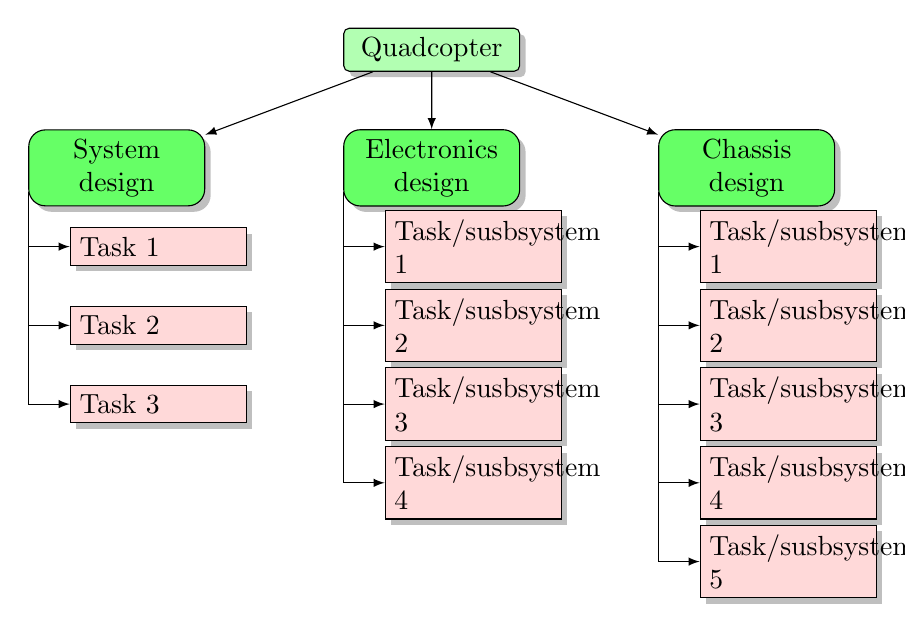
\begin{tikzpicture}[remember picture,level 1/.style={sibling distance=40mm},edge from parent/.style={->,draw},>=latex]

% the initial tree ("root" and "text nodes")
\node[style1] {Quadcopter}
child {node[style2] (c1) {System design}}
child {node[style2] (c2) {Electronics design}}
child {node[style2] (c3) {Chassis design}};

% the nodes below each of the "text" nodes
\node [style3,below of = c1,xshift=15pt] (c11) {Task 1};
\node [style3,below of = c11] (c12) {Task 2};
\node [style3,below of = c12] (c13) {Task 3};

\node [style3,below of = c2,xshift=15pt] (c21) {Task/susbsystem 1};
\node [style3,below of = c21] (c22) {Task/susbsystem 2};
\node [style3,below of = c22] (c23) {Task/susbsystem 3};
\node [style3,below of = c23] (c24) {Task/susbsystem 4};

\node [style3,below of = c3,xshift=15pt] (c31) {Task/susbsystem 1};
\node [style3,below of = c31] (c32) {Task/susbsystem 2};
\node [style3,below of = c32] (c33) {Task/susbsystem 3};
\node [style3,below of = c33] (c34) {Task/susbsystem 4};
\node [style3,below of = c34] (c35) {Task/susbsystem 5};

% lines from each "text" node to every one of its "children"
\foreach \value in {1,2,3}
  \draw[->] (c1.195) |- (c1\value.west);

\foreach \value in {1,...,4}
  \draw[->] (c2.195) |- (c2\value.west);

\foreach \value in {1,...,5}
  \draw[->] (c3.195) |- (c3\value.west);

\end{tikzpicture}
\end{center}

The Gantt chart takes the tasks and subtasks specified in the work break down structure
and schedules when the tasks and subtasks will be commenced and completed as shown below.
Your example should be more detailed than
the example and broken down into subtasks. 
The Gantt chart shown here is done by screenshot-ting a table in excel.  You may use
what ever method you prefer to incorporate your Gantt chart into this report. 

\begin{figure}[!h]
\centering
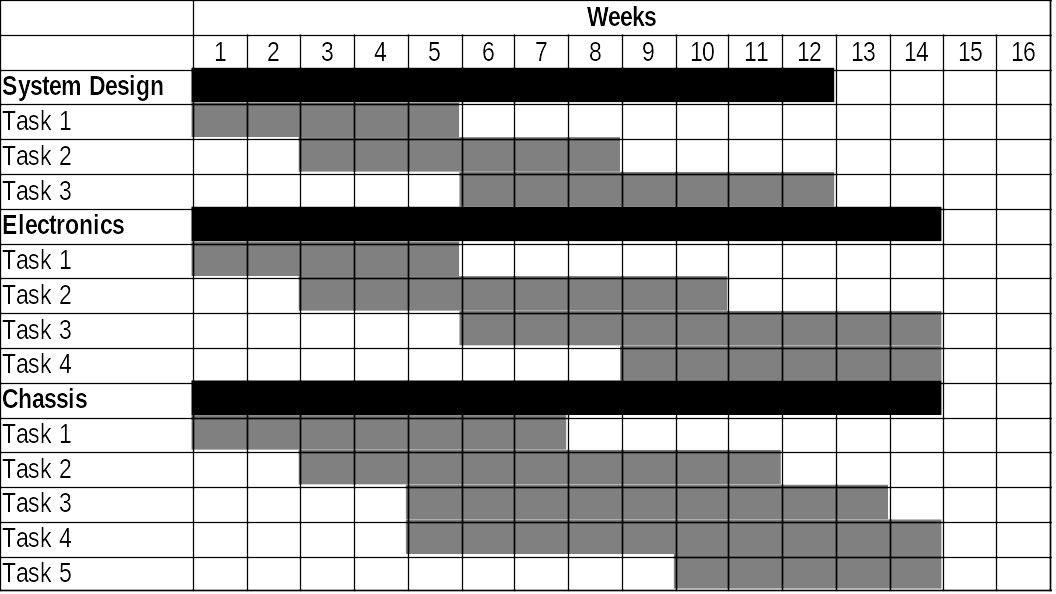
\includegraphics[width=16cm]{Figures/gantt.png}

\caption{Gantt chart}
\label{f.gantt}

\end{figure}


\subsection{Ideation, analysis, and selection}

You must show that in your early design phase you engage in a systematic method whereby 
you generate ideas and then carefully consider and compare them based on their likelihood to
satisfy your design requirements. One tool that you may choose to employ in this subsection
is a decision matrix where you weigh your design ideas based on the likelihood that 
you assess they will satisfy your various design requirements.  You may also use lists
of pros and cons or any of a variety of approaches to choosing between competing ideas.

This subsection should be long enough to fully describe and illustrate
your various design ideas.  You should make use of preliminary cad models in 
this subsection and other nice looking methods of illustrating and explaining
your various design ideas.

\subsection{Design Development}
In this section you chronicle the development of your design both overall
and for each subsystem. This section 
could be broken up into parts of your design and within each
part you should illustrate the progression of your design (with cad
models if appropriate) and discuss mathematical analyses you conducted and prototypes 
you made and tested. Mathematical analyses, simulation, demonstration, and testing
are done for the sole purpose of evaluating a design against
one of your design requirements. You have
to be judicious and determine in what situations which verification methods 
are best.

\section{Results and Discussions}

Presents the data generated in the project relative to the design specifications and objectives 
defined for the project in order to enable an assessment of the success of the project. An 
assessment of the project’s success, with justification, shall be made. Known limitations and 
issues with the design project should be discussed in this section. Significant challenges 
encountered and deviations from the original plan should be included.

\section{Future Work}

Based upon the results obtained, recommended future work related to the process or product 
should be discussed. 

\section{Summary and Conclusion}

A restatement of the objectives of the project and an assessment of the outcome of the project 
relevant to the objectives, including the significance of the work in the design context. 

\section{References}


% Here I am redefining the section command to suppress the generation of a second section titles when \section is called by \begin{thebibliography}

\let\seccs=\section
\renewcommand{\section}[2]{}%

\begin{thebibliography}{20}
%
\bibitem{hibbler} Hibbler RC, {\it Mechanics of Materials}, Upper Saddle River, N.J: Pearson Education, 2003. Print.
%
\end{thebibliography}

%\bibliographystyle{unsrt}
%\bibliography{references}{}

% Here I am restoring the original definition of the section command to generate section titles again
\let\section=\seccs

\section{Appendix}
If applicable, large data sets, collections of photos, and step by step procedures for 
manufacturing materials or conducting tests will be included here. Drawing packets, BOMs,
construction documents, detailed circuit/system diagrams, and code will be stored here. 
Applicable standards may also be attached if they are not excessively long.
Material shall be 
organized into multiple appendices as necessary, using an uppercase alphabetic identifier (
e.g., Appendix A). If an appendix is not required, the section shall be deleted. 

\section{Author contributions}
Writing of  the final design report is intended to be shared by all team members.  
In this section put in your name as the subsection heading and give a summary of 
what you contributed to the writing of the final design project report. 
\subsection{Name of team member 1}
\subsection{Name of team member 2}
\subsection{Name of team member 3}



\end{document}
